% Instructions for submitting the final version ===================================================
%
% Submit at http://www.sheridanprinting.com/acm/icfp/icfp.cfm?id=icfp78n
% NB: Our paper id is "icfp78n"
%
% File name for submission: Then kindly name your .tex and (eventually your final .ps and .pdf
%  files) using your ICFP Paper # with the lead author's last name (example: 
%  icfp456-weaver.tex /icfp456-weaver.pdf --AND-- .ps). Be sure to format your document for
%  American Letter (8-1/2x11).
%
% IMPORTANT: 
% * Include .bbl into the submitted .tex (to provide ACM DL with metadata).
% * Need to use Type 1 fonts and they want us to submit PS, too, as they don't trust
%   our PDF, but I don't think we can produce PS as your figures are in PDF.  I'd say, let's
%   submit PDF only.
% =================================================================================================


% TODO for final version
% ~~~~~~~~~~~~~~~~~~~~~~
% * On page 2, figure 1, the type of sum has no Shape constraint on sh, although it does at the top
%   of page 5.
% * Check that the indicies in mmMult are all ok.
% * Three minor comments
%   - section 3.2 discusses DArray's without them ever being introduced anywhere,
%   - something like Redim or Reshape might be a better name for your Slice class as it is used for
%     both slice and replicate, and
%   - why not have a foldl, foldr, and fold, where the former two are for when order of operations
%     matter, and the latter when they don't.
%   I was also thinking something like the Slice class trick would give a nice way of specifying which
%   dimensions to apply shape polymorphic functions to. That is, instead of having do an index
%   permutation to being the dimensions I wish to operate to the end, it would be nice to be able to
%   just do
%     apply (Any :. 0 :. All) (fold (+)) arr
%   and have the fold apply along the second last dimension.
%
%   The integer could be the seed for the fold, or you could introduce a new empty data type to
%   indicate the dimension). Even more generally, you could make it so a subset of dimensions could be
%   specified for applying multi-dimensional polymorphic functions.
%
% * (DONE [rl]) Regarding that Repa programs parallelise without change, a person on reddit replied that that is
%   mostly the case for C with OpenMP, too IN THE CASES WHERE OPENMP ACTUALLY WORKS.
%   The tricky bit for us is that it works for simple things like matrix multiplication:
%
%     OpenMP is probably the easiest way, if you just want to run iterations of an existing loop in
%     parallel. Slap on a
%     #pragma omp for shared(<arrays>) private(<loop indices>)
%     If you want complete automation, try -parallel with Intel's compilers, if you have access to them.
%
%   My reply was: That's true. A simple kernel like that the Intel compiler should be able to handle.
%   The problem with automatic loop parallelisation is of course that it sometimes works and sometimes
%   it doesn't, just because the compiler couldn't figure out some dependency and can't be sure it is
%   safe to parallelise. In Haskell, it is always safe in pure code (and the compiler knows whether
%   code is pure from its type).
%
%   We may need to address this in related work.


% Suggestions for later:
% ------------------
% data Array sh e where
%   Delayed :: sh -> (sh -> e) -> Array sh e
%   Manifest :: (Shape sh, Elt e) => sh -> UArr e -> Array sh e
% -----------------
% Here is a much nicer type for backpermute
%   backpermute :: (sh -> sh') -> (sh' -> sh) -> Array sh e -> Array sh' e
% Now we can say that in a call
%   backpermute f g, it should be the case that f.g is identity.
% (or the other way round).  And back-permute client code gets nicer I think.
% -----------------
% I'm not sure that 'delay' should return a shape. We already have 'extent' for that
% -----------------
% Could we unify slice and replicate, using a None slice specifier?


%
%  General todos from the reviews 
%

% check that code doesn't run over page, column? review 2

% The double construction in the representation of Array is
% a pattern we see again and again. Perhaps there is something
% more general going on here

% review 2
% You may
% want to include some discussion about the tools and techniques
% that could be used to performance debug array based computations.

%
% Bring out the tool for reaching parallelism, force, in a more explicit way.
% From reading the text, force is the only way to get parallelism. How
% does force make choices about this split, for example?


% The paper fails to clarify the relationship
%   between the presented concepts and "data parallel haskell", deeply
%   woven into GHC-(�=6.13). On page 1, the claim "does not require any
%   compiler support specific to its implementation" is untrue for
%   performance considerations (or not?)


% "Very Bad Indeed" (capitalised) seems to be a common idiom and
%   joke for the authors - but just misplaced to me as a reviewer. (reviewer 3)
% do we want to change this??

% The type given to the crucial function "traverse" does not match
%    its usage (throughout the paper! first in backpermute right below).
%    Clearly the de-facto usage with the array to traverse as the last
%    argument is preferable, but package repa-1.1.0.0 uses the other version.
%    reviewer 3  - already fixed by Ben?

%    Ref [21] (from the same group as the authors) is unspecific, and
%    referenced from text only in a digression. Can be removed.

\documentclass{sigplanconf}

%\usepackage[british]{babel}
\usepackage{version}
\usepackage[pdftex]{graphicx}
\usepackage{amsmath}
\usepackage{amsfonts,amssymb}
\usepackage{url}
\usepackage{alltt}
\usepackage{code}


\renewcommand{\textfraction}{0.2}
\renewcommand{\topfraction}{0.9}
\renewcommand{\dbltopfraction}{0.9}
\renewcommand{\floatpagefraction}{0.9}
\renewcommand{\dblfloatpagefraction}{0.9}

\newcommand{\simon}[1]{\emph{\textbf{SLPJ:} #1}}
\newcommand{\slpj}[1]{\emph{\textbf{SLPJ:} #1}}
\newcommand{\rl}[1]{\emph{\textbf{RL:} #1}}
\newcommand{\gck}[1]{\emph{\textbf{GCK:} #1}}
\newcommand{\manuel}[1]{\emph{\textbf{MMTC:} #1}}
\newcommand{\benl}[1]{\emph{\textbf{BL:} #1}}
\newcommand{\TODO}[1]{\emph{\textbf{TODO:} #1}}
\newcommand{\finaltodo}[1]{\emph{\textbf{TODO FINAL:} #1}}

% \makeatletter
% \def \ps@plain {%
%   \let \@mkboth = \@gobbletwo
%   \let \@evenhead = \@empty
%   \def \@evenfoot { \thepage \hfil \scriptsize \textit{\@preprintfooter}\hfil
%                    \textit{\@formatyear}}%
%   \let \@oddhead = \@empty
%   \let \@oddfoot = \@evenfoot}
% \makeatother

\begin{document}

\preprintfooter{\textbf{--- DRAFT --- DRAFT --- DRAFT --- DRAFT ---}}
\conferenceinfo{ICFP'10,} {September 27--29, 2010, Baltimore, Maryland, USA.}
\CopyrightYear{2010}
\copyrightdata{978-1-60558-794-3/10/09}

\title{Regular, Shape-polymorphic, Parallel Arrays in Haskell}
\authorinfo{
  \shortstack{%
    Gabriele Keller$^\dagger$ \and 
    Manuel M. T. Chakravarty$^\dagger$ \and 
    Roman Leshchinskiy$^\dagger$ 
    \\[4pt]
    Simon Peyton Jones$^\ddagger$ \and
    Ben Lippmeier$^\dagger$ 
  }
}{
  \vspace{5pt}
  \shortstack{
    $^\dagger$Computer Science and Engineering \\
    University of New South Wales, Australia \\[2pt]
    \textsf{\{keller,chak,rl,benl\}@cse.unsw.edu.au}
  }
  \and
  \shortstack{
    $^\ddagger$Microsoft Research Ltd \\
    Cambridge, England \\[2pt]
    \textsf{\{simonpj\}@microsoft.com}
  }
}{%
}
\maketitle

\makeatactive

\begin{abstract}
  We present a novel approach to regular, multi-dimensional arrays in Haskell.
The main highlights of our approach are that it (1) is purely functional, (2)
supports reuse through shape polymorphism, (3) avoids unnecessary intermediate
structures rather than relying on subsequent loop fusion, and (4) supports transparent parallelisation.
  
  We show how to embed two forms of shape polymorphism into Haskell's type system using type classes and type families.  In particular, we discuss the generalisation of regular array transformations to arrays of higher rank, and introduce a type-safe specification of array slices.
  
  We discuss the runtime performance of our approach for three standard array algorithms.  We achieve absolute performance comparable to handwritten C code.  At the same time, our implementation scales well up to 8 processor cores.
\end{abstract}

\category{D.3.3}{Programming Languages}{Language Constructs and Features---Concurrent programming structures; Polymorphism; Abstract data types}
 
\terms
Languages, Performance

\keywords Arrays, Data parallelism, Haskell

% please leave table of contents for the draft
%\tableofcontents\newpage

% ----------------------
\section{Introduction}

In purely functional form, array algorithms are often more elegant
and easier to comprehend than their imperative, explicitly loop-based
counterparts.  The question is, can they also be efficient?

Experience with Clean, OCaml, and Haskell has shown that we can write efficient
code if we sacrifice purity and use an \emph{imperative array interface} based
on reading and writing \emph{individual array elements}, possibly wrapped in
uniqueness types or monads~\cite{groningen:clean-arrays, leroy:ocaml-3.11, 
launchbury:lazy-functional-state-threads}. 
However, using impure features not only obscures clarity, 
but also forfeits the transparent
exploitation of the data parallelism that is abundant in array algorithms. 
% In such programs side effects need to be carefully controlled, 
% and algorithms based on access to individual elements often parallelise poorly.
  
In contrast, using a \emph{purely-functional array interface} based on
\emph{collective operations} ---such as maps, folds, and permutations---
emphasises an algorithm's high-level structure and often has an obvious parallel
implementation. This observation was the basis for previous work on algorithmic
skeletons and the use of the \emph{Bird-Meertens Formalism (BMF)} for parallel
algorithm design~\cite{rabhi-gorlatch:pattyerns-skeletons}. Our own work on
\emph{Data Parallel Haskell (DPH)} is based on the same premise, but aims at
irregular data parallelism which comes with its own set of challenges \cite{peyton-jones-etal:harnessing-multicores}. 
Other work on \emph{byte
arrays}~\cite{coutts-etal:rewriting-haskell-strings} also aims at high-performance, while abstracting
over loop-based low-level code using a purely-functional combinator
library. 

% \simon{A disadvantage of collective operations is that they are rather
% inflexible.  I think a contribution of this paper is that one can still do
% things element-wise, as well as collectively? If so we should highlight
% the tension, and claim to have resolved it (somewhat).  SaC does this too I think, in its
% with-loops.  What's the relative expressiveness of with-loops and our stuff?}
% \manuel{There are many different approach using collective operations; e.g., also in Fortran.  I don't think using permutations etc is new and I wouldn't feel comfortable claiming any novelty in that regard.  Re SaC, difficult to say.  Gabi found that the code is more compact with our operations, but I don't think we have enough data to make a statement that we can support.}

We aim higher by supporting multi-dimensional arrays, more
functionality, and transparent parallelism.
% The questions that we address in this paper are the following: Can a
% purely-functional array interface deliver the same level of performance as an
% imperative array interface? Is this possible with an entirely library-based
% implementation in a lazy general-purpose language? Can we transparently
% parallelise the implementation? The answer to each of the three questions is an
% emphatic yes! 
We present a Haskell library of regular parallel arrays, which we call 
\emph{Repa\footnote{Repa means ``turnip'' in Russian.}}
(Regular Parallel Arrays).  While Repa makes use of
the Glasgow Haskell Compiler's many existing extensions, it is a pure library: 
it does not require any language extensions that are specific to its implementation. The resulting code
is not only as fast as when using an imperative array interface, it 
approaches the performance of handwritten C code, and exhibits good parallel
scalability on the configurations that we benchmarked. 

In addition to good performance, we achieve a high degree of reuse by supporting
\emph{shape polymorphism}.
For example, \texttt{map} works over arrays of arbitrary rank, while \texttt{sum} 
decreases the rank of an arbitrary array by one -- we give more details
in Section~\ref{sec:shape-poly}.
The value of shape polymorphism has been demonstrated by the language 
Single Assigment C, or SAC ~\cite{scholz:SaC}. Like us, SAC aims at
purely functional high-performance arrays, but  SAC is
a specialised array language based on a purpose-built compiler. We show
how to embed shape polymorphism into Haskell's type system. 

The main contributions of the paper are the following:
%
\begin{itemize}
\item An API for purely-functional, collective operations over dense, 
  rectangular, multi-dimensional arrays supporting shape polymorphism
  (Section~\ref{sec:API}).
\item Support for various forms of constrained shape polymorphism in a
  Hindley-Milner type discipline with type classes and type families
  (Section~\ref{sec:shape-poly}).
\item An aggressive loop fusion scheme based on a functional 
  representation of delayed arrays (Section~\ref{sec:fusion}).
\item A scheme to transparently parallelise array algorithms based on our API 
  (Section~\ref{sec:parallelism})
\item An evaluation of the sequential and parallel performance of our approach
  on the basis of widely used array algorithms (Section~\ref{sec:benchmarks}).
\end{itemize}
%
Before diving into the technical details of our contributions, the next section
illustrates our approach to array programming by way of an example.

% ----------------------
\section{Our approach to array programming} \label{sec:overview}
\label{sec:rarraylib} \label{s:mmMult} 

A simple operation on two-dimensional matrices is transposition. With
our library we express transposition 
in terms of a permutation operation that swaps
the row and column indices of a matrix:
%
\begin{code}
transpose2D :: Elt e => Array DIM2 e -> Array DIM2 e
transpose2D arr 
  = backpermute new_extent swap arr
  where swap (Z :.i :.j) = Z :.j :.i
        new_extent       = swap (extent arr)
\end{code}
%
Like Haskell 98 arrays, our array type is 
parameterised by the array's \emph{index type}, here @DIM2@, 
and by its element type @e@. The index type gives
the \emph{rank} of the array, which we also call 
the array's \emph{dimensionality}, or \emph{shape}.

Consider the type of @backpermute@, given in Figure~\ref{fig:lib-types}.
The first argument is the bounds (or \emph{extent}) 
of the result array, which we obtain by swapping the row and column extents of
the input array. 
For example transposing a $3 \times 12$ matrix gives a
$12 \times 3$ matrix.\footnote{For now, just read the notation @(Z :.i :.j)@ as if
it was the familiar pair @(i,j)@. The details are in Section~\ref{sec:shape-poly} 
where we discuss shape polymorphism.}
The @backpermute@ function constructs a new array in terms of an 
existing array solely through an \emph{index transformation}, supplied as its
second argument, @swap@: given an index into the
result matrix, @swap@ produces the corresponding index into the argument matrix.

A more interesting example is matrix-matrix multiplication:
%
\begin{code}
mmMult :: (Num e, Elt e)
       => Array DIM2 e -> Array DIM2 e
       -> Array DIM2 e
mmMult arr brr 
 = sum (zipWith (*) arrRepl brrRepl)
 where
  trr     = transpose2D brr
  arrRepl = replicate (Z :.All   :.colsB :.All) arr 
  brrRepl = replicate (Z :.rowsA :.All   :.All) trr               
  (Z :.colsA :.rowsA) = extent arr
  (Z :.colsB :.rowsB) = extent brr
\end{code}
%
The idea is to expand both rank-two argument arrays into rank-three arrays by
replicating them across a new dimension, or axis, as illustrated in
Figure~\ref{fig:mmMult}.  The front face of the cuboid represents the array
\texttt{arr}, which we replicate as often as \texttt{brr} has columns
(\texttt{colsB}), producing @arrRepl@.  The top face represents @trr@
(the transposed @brr@), which we replicate as often as \texttt{arr}
has rows (\texttt{rowsA}), producing @brrRepl@.  As indicated by the
figure, the two replicated arrays have the same extent, which
corresponds to the index space of matrix multiplication:
\[
(AB)_{i,j}=\Sigma^n_{k=1}A_{i,k}B_{k,j}
\]
where $i$ and $j$ correspond to @rowsA@ and @colsB@ in our code.  The summation index $k$ corresponds to the innermost axis of the replicated arrays and to the  left-to-right axis in Figure~\ref{fig:mmMult}.  Along this axis we perform the summation after an elementwise multiplication of the replicated elements of @arr@ and @brr@ by @zipWith (*)@.
%
% NB: Don't move foward!  We want the figures in the second column on Page 2.
\begin{figure}
\begin{code}
extent  :: Array sh e -> sh

sum     :: (Shape sh, Elt e, Num e)
        => Array (sh :. Int) e -> Array sh e

zipWith :: (Shape sh, Elt e1, Elt e2, Elt e3)
        => (e1 -> e2 -> e3)
        -> Array sh e1 -> Array sh e2
        -> Array sh e3

backpermute :: (Shape sh, Shape sh', Elt e)
            => sh' -> (sh' -> sh)
            -> Array sh e -> Array sh' e
\end{code}
\caption{Types of library functions} \label{fig:lib-types}
\end{figure}
%
\begin{figure} 
  \centering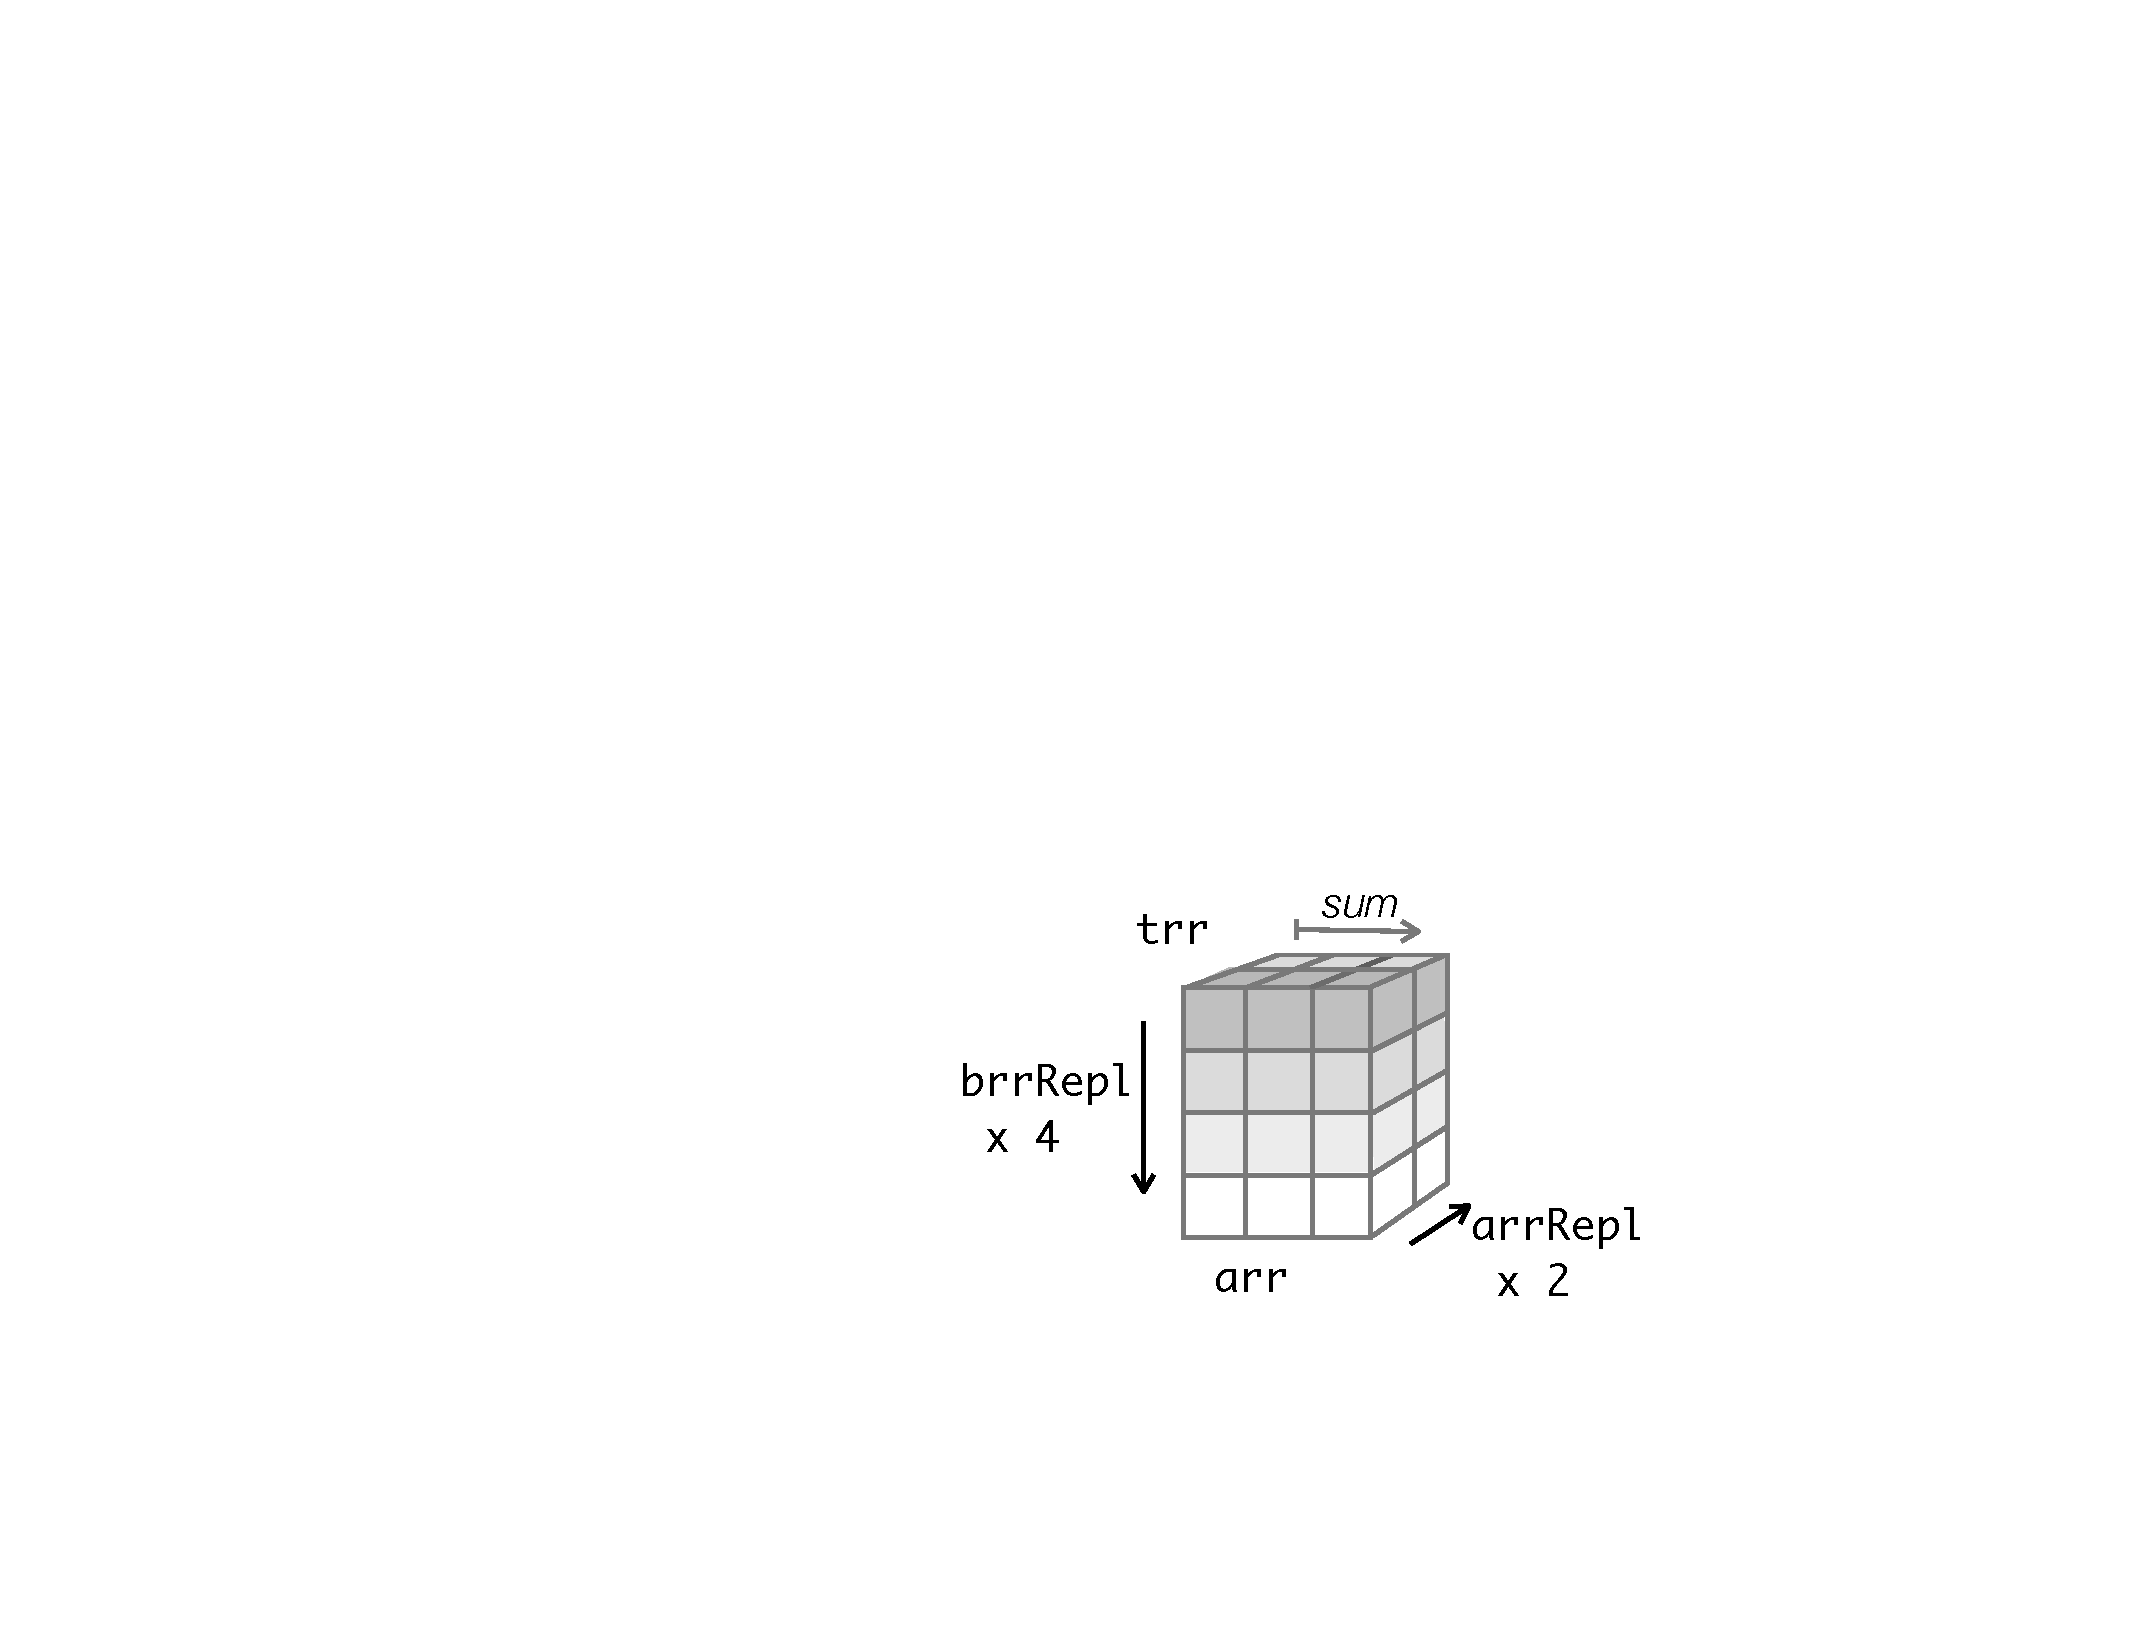
\includegraphics[width=0.3\textwidth]{figs/MatrixDiagram.pdf}
%  \includegraphics[width=0.6\textwidth]{./Matrixmult-arr.pdf} 
  \caption{Matrix-matrix multiplication illustrated} 
  \label{fig:mmMult} 
\end{figure}

A naive implementation of the operations used in \texttt{mmMult} would result in very bad space and time performance. In particular, it would be very inefficient to compute explicit representations of the replicated matrices \texttt{arrRepl} and \texttt{brrRepl}. Indeed, a key principle of our design is to avoid generating explicit representations of the intermediate arrays that can be represented as the original arrays combined with a \emph{transformation of the index space} (Section~\ref{sec:delayed_arrays}). 
A rigorous application of this principle results in aggressive loop fusion
(Section~\ref{sec:fusion}) producing code that is similar to imperative code.
As a consequence, this Haskell code has about the same performance as
handwritten C code for the same computation. Even more importantly, we
measured very good absolute speedup, \(\times7.2\) for 8 cores, on multicore
hardware. For the C code, this can only be achieved through considerable
additional effort or by employing special-purpose language extensions such as
OpenMP~\cite{openmp:spec} which often have difficulties with more complex programs.

% -----------------------------------------
\section{Representing arrays} \label{sec:representation}

The representation of arrays is a central issue in any array library.
Our library uses two devices to achieve good performance:
%
\begin{enumerate}
\item We represent array data as contiguously-allocated ranges of \emph{unboxed} values.
\item We \emph{delay} the construction of intermediate arrays to support constant-time index transformations and slices, and to combine these operations with traversals over successive arrays.
\end{enumerate}
%
We describe these two techniques in the following sections.

\subsection{Unboxed arrays} \label{sec:unboxed}

In Haskell 98 arrays are lazy: each element of an array
is evaluated only when the array is indexed at that position.
Although convenient, laziness is Very Bad Indeed for array-intensive programs:
\begin{itemize}
\item A lazy array of (say) @Float@ is represented as an array of pointers
to either heap-allocated thunks, or boxed @Float@ objects, depending on whether
they have been forced.
This representation requires at least three times as much storage as a 
conventional, contiguous array of unboxed floats. Moreover, when
iterating through the array, the lazy representation imposes higher memory traffic.
This is due to the increased size of the individual elements, as well as their
lower spacial locality.
\item In a lazy array, evaluating one element does not mean that the other
elements will be demanded.  However, the overwhelmingly common case is that the 
programmer intends to demand the entire array, and wants it evaluated in parallel.
\end{itemize}
We can solve both of these problems simultaneously using a Haskell-folklore
trick. We define a new data type of arrays, which we
will call @UArr@, short for ``unboxed array''.  
These arrays are \emph{one-dimensional}, indexed by @Int@,
and are slightly stricter than Haskell~98 arrays:
a @UArr@ \emph{as a whole} is evaluated lazily, but 
an attempt to evaluate any \emph{element} of the array (e.g. by indexing) 
will cause evaluation of all the others, in parallel.

For the sake of definiteness we give a bare sketch of how @UArr@ is
implemented.  However, this representation is not new; it is well
established in the Haskell folklore, and we use it in Data Parallel
Haskell (DPH)~\cite{peyton-jones-etal:harnessing-multicores,chak-etal:DPH}, so we do not elaborate the details.
%
\begin{quote}
\begin{code}
class Elt e where
  data UArr e
  (!) :: Array e -> Int -> e
  ...more methods...

instance Elt Float where
  data UArr Float = UAF Int ByteArray#
  (UAF max ba) ! i 
     | i < max   = F# (indexByteArray ba i)
     | otherwise = error "Index error"
  ...more methods...

instance (Elt a, Elt b) => Elt (a :*: b) where
  data UArr (a :*: b) = UAP (UArr a) (UArr b)
  (UAP a b) ! i = (a!i :*: b!i)
  ...more methods...
\end{code}
\end{quote}
%
Here we make use of Haskell's recently added \emph{associated data types}~\cite{chak-etal:ATs} to represent an array of @Float@ as a contiguous array of unboxed floats (the @ByteArray#@), and an array of pairs as a pair of arrays.  Because the representation of the array depends on the element type, indexing must vary with the element type too, which explains why the indexing operation @(!)@ is in a type class @Elt@.

In addition to an efficient
underlying array representation, we also need the infrastructure to
operate on these arrays in parallel, using multiple processor cores.
To that end we reuse part of our own parallel array
library of Data Parallel Haskell. This provides us with an optimised
implementation of @UArr@ and the @Elt@ class, and with 
parallel collective operations over @UArr@.  It also requires us to represent pairs using the strict pair constructor @(:*:)@, instead of Haskell's conventional @(,)@.


\subsection{Delayed arrays}
\label{sec:delayed_arrays}

When using Repa, index transformations such as @transpose2D@ (discussed in Section \ref{sec:rarraylib}) are ubiquitous. As we expect index transformations to be cheap, it would be wrong to (say) copy a 100Mbyte array just to transpose it. It is much better to push the index transformation into the consumer, which can then consume the original, unmodified array.

We could do this transformation statically, at compile time, 
but doing so would rely on the consumer being able to ``see'' the 
index transformation. This could make it hard for the programmer to predict whether 
or not the optimisation would take place. In Repa 
we instead perform this optimisation dynamically, and offer a guarantee that
index transformations perform no data movement.  The idea is simple and well known:
%\simon{Can we cite pointers?}
just represent an array by its indexing  function, together with the array 
bounds (this is not our final array representation):
%
\begin{quote}
\begin{code}
data DArray sh e = DArray sh (sh -> e)
\end{code}
\end{quote}
%
With this representation, functions like @backpermute@ 
(whose type signature appeared in Figure~\ref{fig:lib-types}) are quite easy to implement:
\begin{quote}
\begin{code}
backpermute sh' fn (Array sh ix1)
  = Array sh' (ix1 . fn)
\end{code}
\end{quote}
%
We can also wrap a @UArr@ as a @DArray@:
%
\begin{quote}
\begin{code}
wrap :: (Shape sh, Elt e) 
     => sh -> UArr e -> DArray sh e
wrap sh uarr  = Array sh idx
  where idx i = uarr ! toIndex sh i
\end{code}
\end{quote}
%
When wrapping an @DArray@ over a @UArr@, we also take the opportunity to
generalise from one-dimensional
to multi-dimensional arrays.  The index of these multi-dimensional arrays is of type @sh@,
where the @Shape@ class (to be described in Section~\ref{sec:shape-class}) 
includes the method @toIndex :: Shape sh => sh -> sh -> Int@.
This method maps the bounds and index of an @Array@ to the corresponding linear @Int@ index
in the underlying @UArr@. 

% -----------------------------------------------------------------------------
\subsection{Combining the two}
\label{sub:combining_the_two}

Unfortunately, there are at least two reasons why it is not always beneficial to
delay an array operation.  One is \emph{sharing}, which we discuss later
in Section~\ref{sec:fusion}.  Another is \emph{data layout}. In our @mmMult@ example from Section \ref{s:mmMult}, we want to delay the two applications of @replicate@, but not the application of @transpose2D@.  Why?  We store multi-dimensional arrays in row-major order (the same layout Haskell 98 uses for standard arrays).  Hence, iterating over the second index of an array of rank 2 is more cache friendly than iterating over its first index.

It is well known that the order of the loop nest in an imperative implementation of matrix-matrix multiplication has a dramatic effect on performance due to these cache effects.  By forcing @transpose2D@ to produce its result as an unboxed array in memory ---we call this a \emph{manifest} array--- instead of leaving it as a delayed array, the code will traverse both matrices by iterating over the second index in the inner loop.  Overall, we have the following implementation:
%
\begin{code}
mmMult arr brr
 = sum (zipWith (*) arrRepl brrRepl)
 where
  trr     = force (transpose2D brr)  -- New! force!
  arrRepl = replicate (Z :.All   :.colsB :.All) arr
  brrRepl = replicate (Z :.rowsA :.All   :.All) trr             

  (Z :.colsA :.rowsA) = extent arr
  (Z :.colsB :.rowsB) = extent brr
\end{code}  

We could implement @force@ by having it produce a value of type @UArr@ and then apply @wrap@ to turn it into a @DArray@ again, providing the appropriate memory layout for a cache-friendly traversal.  This would work, but we can do better.  The function @wrap@ uses array indexing to access the underlying @UArr@.  In cases where this indexing is performed in a tight loop, GHC can optimise the code more thoroughly when it is able to inline the indexing operator, instead of calling an anonymous function encapsulated in the data type @DArray@. For recursive functions, this also relies on the \emph{constructor specialisation} optimisation~\cite{peyton-jones:constructor-specialisation}.  However, as explained in~\citet[Section~7.2]{coutts-etal:stream-fusion}, to allow this we must make the special case of a wrapped @UArr@ explicit in the datatype, so the optimiser can see whether or not it is dealing directly with a manifest array.

Hence, we define regular arrays as follows:
%
\begin{quote}
\begin{code}
data Array sh e = Manifest sh (UArr e)
                | Delayed  sh (sh -> e)
\end{code}
\end{quote}
%
We can unpack an arbitrary @Array@ into delayed form thus:
%
\begin{quote}
\begin{code}
delay :: (Shape sh, Elt e) 
      => Array sh e -> (sh, sh -> e)
delay (Delayed  sh f)    = (sh, f)
delay (Manifest sh uarr) 
      = (sh, \i -> uarr ! toIndex sh i)
\end{code}
\end{quote}
%
This is the basis for a general @traverse@ function that produces a delayed array after applying a transformation. 

%\pagebreak{}
The transformation produced with @traverse@ may include index space transformations or other computations:
%
\begin{quote}
\begin{code}
traverse :: (Shape sh, Shape sh', Elt e)
         => Array sh e 
         -> (sh -> sh') 
         -> ((sh -> e) -> sh' -> e')
         -> Array sh' e'
traverse arr sh_fn elem_fn 
  = Delayed (sh_fn sh) (elem_fn f)
  where (sh, f) = delay arr
\end{code}
\end{quote}
We use @traverse@ to implement many of the other operations of our library --- for example, @backpermute@ is implemented as:
%
\begin{quote}
\begin{code}
backpermute :: (Shape sh, Shape sh', Elt e)
            => sh' -> (sh' -> sh) -> Array sh e 
            -> Array sh' e
backpermute sh perm arr 
  = traverse arr (const sh) (. perm) 
\end{code}
\end{quote}
%
We discuss the use of @traverse@ in more detail in Sections~\ref{sec:API} \&~\ref{sec:parallelism}.

% subsection combining_the_two (end)



% -----------------------------------------------
\section{Shapes and shape polymorphism} 
\label{sec:shape-poly}
\label{sec:shape-class}

In Figure~\ref{fig:lib-types} we gave this type for @sum@:
%
\begin{quote}
\begin{code}
sum :: (Shape sh, Num e, Elt e) 
    => Array (sh:.Int) e -> Array sh e
\end{code}
\end{quote}
As the type suggests, @sum@ 
is a \emph{shape-polymorpic} function: it can sum the
rightmost axis of an array of arbitrary rank.  In this section
we describe how shape polymorphism works in Repa.
We will see that combination of parametric polymorphism, type classes, and type
families enables us to track the rank of each array in its type, 
guaranteeing the absence of rank-related runtime errors.
We can do this even in the presence of operations such as slicing and
replication which change the rank of an array.
However, bounds checks on indices are still performed at
runtime --- tracking them requires more sophisticated type system
support~\cite{xi:dml,swierstra-altenkirch:dep-types-for-distr-arrays}.

\begin{figure}
  \centering
\begin{code}
infixl 3 :.
data Z            = Z
data tail :. head = tail :. head

type DIM0 = Z
type DIM1 = DIM0 :. Int
type DIM2 = DIM1 :. Int
type DIM3 = DIM2 :. Int

class Shape sh where
 rank    :: sh -> Int
 size    :: sh -> Int       -- Number of elements
 toIndex :: sh -> sh -> Int -- Index into row-major
 fromIndex                  --   representation
         :: sh -> Int -> sh -- Inverse of 'toIndex'
 <..and so on..>
  
instance             Shape Z         where ...
instance Shape sh => Shape (sh:.Int) where ...
\end{code}
  \caption{Definition of shapes}
  \label{fig:shapes}
\end{figure}
%
\subsection{Shapes and indices}
% \finaltodo{ 4.1 can be reorganised as follows: starting by the part "The
%   extent of an array..", then introducing the representation as snoc
%   lists, then discussing/mentioning Ix.  Also, the paper should point
%   at "instance Shape sh =� Shape (sh:.Int)" as the main motivation
%   for an extra data type.'  do we want to change this??? reviewer 3}

Haskell's tuple notation does not allow us the flexibility we need, so we introduce our own notation
for indices and shapes. As defined in Figure~\ref{fig:shapes}, we use an inductive notation of tuples
as heterogenous \emph{snoc} lists. On both the type-level and the value-level, we use 
the infix operator \texttt{(:.)} to represent \emph{snoc}. The constructor @Z@ corresponds to a rank zero shape, and we use it to mark the end of the list.
Thus, a three-dimensional index with components \texttt{x},
\texttt{y} and \texttt{z} is written \texttt{(Z:.x:.y:.z)} and has type
\texttt{(Z:.Int:.Int:.Int)}. This type is the \emph{shape} of the array.
Figure~\ref{fig:shapes} gives type synonyms for common shapes: 
a singleton array of shape @DIM0@ represents a scalar value; an array of shape @DIM1@ is 
a vector, and so on.

% We are forced to use snoc lists, rather than the more conventional cons
% lists, because only snoc lists allow row-major storage of multi-dimensional arrays,
% and the use of row-major arrays is prescribed by the Haskell 98 language
% standard for the standard array type. To avoid confusion and to ensure the
% efficient conversion between different types of arrays, we follow the
% storage layout fixed in standard. \simon{At this point it is absolutely unclear
% why H98 forces snoc}
%
% We use snoc lists so that we can follow the universal convention that
% \manuel{It is not universal, Fortran and MatLab are the famous exceptions.}
The motivation for using \emph{snoc} lists, rather than the more conventional \emph{cons} lists, is this:
we store manifest arrays in row-major order, where the \emph{rightmost} index is the most \emph{rapidly-varying} when traversing linearly over the array in memory. For example, the value at index \texttt{(Z:.3:.8)} is stored adjacent to that at \texttt{(Z:.3:.9)}.  This is the same convention adopted by Haskell 98 standard arrays.

We draw array indices from \texttt{Int} values only, so the shape
of a rank-$n$ array is:
\[
\texttt{Z }\underbrace{\texttt{:. Int :. $\cdots$ :. Int}}_{\text{$n$ times}}
\]
In principle, we could be
more general and allow non-@Int@ indices, like Haskell's index type class \texttt{Ix}. However, this
would complicate the library and the presentation, and is orthogonal to the
contributions of this paper; so we do not consider it here. Nevertheless, 
shape types, such as \texttt{DIM2} etc, explicitly mention the \texttt{Int} type. 
This is for two reasons: firstly, it simplifies the transition to using the \texttt{Ix} class if
that is desired; and secondly, in Section~\ref{sec:slices} we discuss 
more elaborate shape constraints that require an explicit index type. 

The \emph{extent} of an array is a value of the shape type:
%
\begin{quote}
\begin{code}
extent :: Array sh e -> sh
\end{code}
\end{quote}
%
The corresponding Haskell 98 function, @bounds@, returns an upper and lower bound,
whereas @extent@ returns only the upper bound. Repa uses zero-indexed arrays
only, so the lower bound is always zero.
For example, the extent \texttt{(Z:.4:.5)} characterises a \(4\times 5\) array of 
rank two containing 20 elements.  The extent along each axis must be at least one.

The shape type of an array also types its indices, which range between
zero and one less than the extent along the same axis.  In other
words, given an array with shape \texttt{(Z:.$n_1$:.$\cdots$:.$n_m$)},
its index range is from \texttt{(Z:.0:.$\cdots$:.0)} to
\texttt{(Z:.$n_1-1$:.$\cdots$:.$n_m-1$)}.  As indicated in
Figure~\ref{fig:shapes}, the methods of the \texttt{Shape} type class
determine properties of shapes and indices, very like Haskell's @Ix@ class.  
These methods are used to
allocate arrays, index into their row-major in-memory representations, 
to traverse index spaces, and are entirely as expected, so we omit
the details.

% -----------------------------------------------------------------------------
\subsection{Shape polymorphism}
% \finaltodo{Consider merging 4.2 and the first part of 4.3. The part following
%   the sum2 example discusses limitations. One of them being that
%   repa does not perform bounds checks (A pathologic
%   shape-polymorphic "filter" version would type-check and even work
%   in checked contexts).}
We call functions that operate on a variety of shapes \emph{shape polymorphic.}
Some such functions work on arrays of any shape at all.  For example, 
here is the type of @map@:
%
\begin{quote}
\begin{code}
map :: (Shape sh, Elt a, Elt b) 
    => (a -> b)
    -> Array sh a -> Array sh b
\end{code}
\end{quote}
%
The function \texttt{map} applies its functional argument to all elements of an array without any concern for the shape of the array.  The type class constraint \texttt{Shape sh} merely asserts that the type variable \texttt{sh} ought to be a shape.  It does not constrain the shape of that shape in any way.

% \simon{There was a Shape type-class constraint here, but I removed it;
% in other places you dont have it.  But you do need an Elt constraint for map, don't you?}
%   \manuel{We now need Elt and Shape constraints due to the new Array definition.}
% Although both these functions are shape-polymorphic, their cost model differs,
% as we mentioned in Section~\ref{sec:delayed}:
% @backpermute@ is an index transformation, 
% implemented as a constant-time operation which leaves
% the underlying data undisturbed;
% but @map@ does real work, and does so in parallel.
% \simon{Is map parallel?}
% \manuel{No, map and backpermute are no different.  Both are implemented by traverse and constant time.  Only when force is applied to the result is any real work performed and then both are equally parallel.  Consequently, I don't think it helps to have both map and backpermute here.}


\subsection{At-least constraints and rank generalisation}
\label{sec:at-least-rank} \label{sec:rank-gen}

With indices as \emph{snoc} lists, we can impose a lower bound on the rank
of an array by fixing a specific number of lower dimensions, but keeping the tail
of the resulting \emph{snoc} list variable. 
%\pagebreak{}
For example, here is the type of @sum@:
%
\begin{quote}
\begin{code}
sum :: (Shape sh, Num e, Elt e) 
    => Array (sh:.Int) e -> Array sh e
\end{code}
\end{quote}
%
This says that @sum@ takes an array of any rank $n\geq1$ and 
returns an array of rank $n-1$.
For a rank-1 array (a vector), @sum@ adds up the vector to return a scalar.
But what about a rank-2 array?  In this case, @sum@ adds up all the rows of the matrix
\emph{in parallel}, returning a vector of the sums.
Similarly, given a three-dimensional array @sum@ adds up each row of 
the array in parallel, returning a two-dimensional array of sums.

Functions like @sum@ impose a lower bound on the rank of an array.  We
call such constraints shape polymorphic \emph{at-least constraints.}
Every shape-polymorphic function with an at-least constraint is
implicitly also a data-parallel map over the unspecified dimensions.
This is a major source of parallelism in Repa.  We call the process of
generalising the code defined for the minimum rank to higher ranks
\emph{rank generalisation.}

The function @sum@ only applies to the rightmost index of an array. What if
we want to reduce the array across a different dimension?  In that case 
we simply perform an index permutation, which is guaranteed cheap,
to bring the desired dimension to 
the rightmost position:
%
\begin{code}
sum2 :: (Shape sh, Elt e, Num e)
     => Array (sh:.Int:.Int) e -> Array (sh:.Int) e
sum2 a = sum (backpermute new_extent swap2 a)
  where 
   new_extent           = swap2 (extent a)
   swap2 (is :.i2 :.i1) = is :.i1 :.i2
\end{code}
%
In our examples so far, we have sometimes returned arrays of a different rank than the input,
but their extent in any one dimension has always been unchanged. 
However, shape-polymorphic functions can also change the extent:
%
\begin{code}
selEven :: (Shape sh, Elt e) 
        => Array (sh:.Int) e -> Array (sh:.Int) e
selEven arr = backpermute new_extent expand arr
  where
   (ns :.n)        = extent arr
   new_extent      = ns :.(n `div` 2)
   expand (is :.i) = is :.(i * 2)
\end{code}
%
As we can see from the calculation of @new_extent@, the array 
returned by @selEven@ is half as big as the input array, in the 
rightmost dimension.
The index calculation goes in the opposite direction, selecting
every alternate element from the input array.

Note carefully that the extent of the new array 
is calculated from the extent of the old array, \emph{but not 
from the data in the array}.  This guarantees we can do rank 
generalisation and still have a rectangular array. To see the difference, consider:
%
\begin{quote}
\begin{code}
filter :: Elt e => (e -> Bool) 
       -> Array DIM1 e -> Array DIM1 e
\end{code}
\end{quote}
%
The @filter@ function is not, and cannot be, shape-polymorphic.  If
we filter each row of a matrix based on the element values, then each new
row may have a different length. This gives no guarantee that the 
resulting matrix is rectangular. In contrast, we have carefully chosen
our shape-polymorphic primitives to guarantee the rectangularity of the output.

\begin{figure}[tp!]
\begin{code}
data All    = All
data Any sh = Any

type family   FullShape ss
type instance FullShape Z    = Z
  ... FullShape (Any sh)     = sh
  ... FullShape (sl :. Int)  = FullShape sl :. Int
  ... FullShape (sl :. All)  = FullShape sl :. Int

type family   SliceShape ss
type instance SliceShape Z   = Z
  ... SliceShape (Any sh)    = sh
  ... SliceShape (sl :. Int) = SliceShape sl
  ... SliceShape (sl :. All) = SliceShape sl :. Int

class Slice ss where
 sliceOfFull:: ss -> FullShape ss  -> SliceShape ss
 fullOfSlice:: ss -> SliceShape ss -> FullShape  ss

instance Slice Z        where ...
instance Slice (Any sh) where ...

instance Slice sl => Slice (sl :. Int) where
  sliceOfFull (fsl :. _) (ssl :. _)	
   = sliceOfFull fsl ssl

  fullOfSlice (fsl :. n) ssl		
   = fullOfSlice fsl ssl :. n

instance Slice sl => Slice (sl :. All) where	
  sliceOfFull (fsl :. All) (ssl :. s)
   = sliceOfFull fsl ssl :. s

  fullOfSlice (fsl :. All) (ssl :. s)
   = fullOfSlice fsl ssl :. s

replicate :: ( Slice sl, Elt e
             , Shape (FullShape sl)
             , Shape (SliceShape sl))
          => sl -> Array (SliceShape sl) e
                -> Array (FullShape sl) e
replicate sl arr
 = backpermute (fullOfSlice sl (extent arr)) 
               (sliceOfFull sl) arr

slice    :: ( Slice sl, Elt e
            , Shape (FullShape sl)
            , Shape (SliceShape sl))
         => Array (FullShape sl) e 
         -> sl -> Array (SliceShape sl) e
slice arr sl
 = backpermute (sliceOfFull sl (extent arr))
               (fullOfSlice sl) arr
\end{code}
\caption{Definition of slices}
\label{fig:slices}
\end{figure}


\subsection{Slices and slice constraints} \label{sec:slices}

% \begin{figure}[tp]
%  \centering
% \begin{code}
% data All    = All
% data Any sh = Any
% 
% class Slice ss where
%   type FullShape  ss
%   type SliceShape ss
%   replicate :: Elt e
%             => ss
%            -> Array (SliceShape ss) e
%             -> Array (FullShape  ss) e
%   slice     :: Elt e
%             => Array (FullShape  ss) e
%             -> ss
%             -> Array (SliceShape ss) e  
%   
% instance Slice Z where
%   type FullShape  Z = Z
%   type SliceShape Z = Z
%   <..definition of replicate and slice omitted..>
% 
% instance Slice (Any sh) where
%   type FullShape  (Any sh) = sh
%   type SliceShape (Any sh) = sh
%   replicate Any a = a
%   slice a Any = a
% 
% instance (Shape (FullShape sl), Shape (SliceShape sl),
%           Slice sl) => Slice (sl:.Int) where
%   type FullShape  (sl:.Int) = FullShape  sl :. Int
%   type SliceShape (sl:.Int) = SliceShape sl
% 
%   replicate (sl:.i) arr 
%      = backpermute (ex:.i) drop arr2 
%      where
%        ex   = extent arr2
%        arr2 = replicate sl arr
%        drop (is:._) = is
% 
%   slice arr (sl:.i) = slice arr2  sl
%      where
%        arr2    = backpermute ex add arr
%        (ex:._) = extent arr 
%        add is  = is:.i
% 
% instance Slice ss => Slice (ss:.All) where
%   type FullShape  (ss:.All) = FullShape  ss :. Int
%   type SliceShape (ss:.All) = SliceShape ss :. Int
%   <..definition of replicate and slice omitted..>
% \end{code}
%   \caption{Definition of slices}
%   \label{fig:slices}
% \end{figure}
%
% \finaltodo{ I got lost in the explanations for the Slice class, unable to match them
%   with code in Fig.4. Giving the instance involving "All" is the minimum
%   to allow readers to figure out functionality from the usage in mmMult.
%   And, the "real code" in repa-1.1.0.0 looks completely different!   review 3}

Shape types characterise a \emph{single} shape. However, some collective array
operations require a relationship between \emph{pairs} of shapes. One
such operation is \texttt{replicate}, which we used in \texttt{mmMult}. The
function \texttt{replicate} takes an array of arbitrary rank and replicates it along
one or more additional dimensions. Note that we cannot uniquely determine the behaviour of
\texttt{replicate} from the shape of the original and resulting arrays alone. For
example, suppose that we want to expand a rank-2 array into
a rank-3 array.  There are three ways of doing this, depending on which dimension of
the resulting array is to be duplicated.
Indeed, the two calls to \texttt{replicate} in \texttt{mmMult} performed
replication along two different dimensions, corresponding to different
sides of the cuboid in Figure~\ref{fig:mmMult}. 

It should be clear that @replicate@ needs an additional argument, a
\emph{slice specifier}, that expresses exactly how the shape of the result
array depends on the shape of the argument array.
A slice specifier has the same format as an array index, but
some index positions may use the value @All@ instead of a
numeric index.
%
\begin{quote}
\begin{code}
data All = All
\end{code}
\end{quote}
%
In \texttt{mmMult}, we use \mbox{\texttt{replicate (Z:.All:.colsB:.All) arr}} to
indicate that we replicate
\texttt{arr} across the second innermost axis, \texttt{colsB} times.  We 
use \texttt{replicate (Z:.rowsA:.All:.All) trr} to specify that we 
replicate \texttt{trr} across the outermost axis, \texttt{rowsA} times.  

The type of the slice specifier \texttt{(Z :.All :.colsB :.All)} is
\texttt{(Z :.All :.Int :.All)}. This type is sufficiently expressive to
determine the shape of \emph{both} the original array, before it gets replicated,
\emph{and} of the replicated array. More precisely, both of these
types are a function of the slice specifier type.
In fact, we derive these shapes using \emph{associated type 
families}, a recent extension to the Haskell type
system~\cite{chak-etal:at-syns,schrijivers-etal:tc-tyfuns}, using the definition
for the @Slice@ type class shown in Figure~\ref{fig:slices}.

A function closely related to @replicate@ is @slice@, which extracts a slice along multiple
axes of an array. The full types of @replicate@ and @slice@ appear in 
Figure~\ref{fig:slices}.
We chose their argument order to match that used for lists:
@replicate@ is a generalisation of @Data.List.replicate@, while @slice@ is a
generalisation of @Data.List.(!!)@.

Finally, to enable rank generalisation for @replicate@ and @slice@, we
add a last slice specifier, namely @Any@, which is also defined in
Figure~\ref{fig:slices}.  It is used in the tail position of a slice,
just like @Z@, but gives a shape variable for rank generalisation.
With its aid we can write @repN@ which replicates an arbitrary array @n@ 
times, with the replication being on the rightmost dimension of the result array:
\begin{quote}
\begin{code}
repN :: Int -> Array sh e -> Array (sh:.Int) e
repN n a = replicate (Any:.n) a
\end{code}
\end{quote}

%    SLPJ: seems superfluous
% In summary, our approach to array programming supports a variety of different
% types of shape polymorphism. Shapes can be unconstrained, as in the signature of
% \texttt{map}, with the type class \texttt{Shape} categorising all
% admissible shapes. Alternatively, shapes can be constrained to be at least of a
% particular rank, as in the signature of \texttt{sum}.
% Finally, two shapes can be constrained such that one of the shapes constitutes a
% specific slice of the second shape, as in the signatures of \texttt{replicate}
% and \texttt{slice}. Here, we use slice specifiers characterised
% by the type class \texttt{Slice} to relate the two shapes.

% --------------------------------------------------------
\section{Rectangular arrays, purely functional} \label{sec:API}

As mentioned in Section~\ref{sec:representation}, the type class @Elt@ determines the set of types that can be used as array elements. We adopt @Elt@ from the library of unboxed one-dimensional arrays in Data Parallel Haskell. With this library, array elements can be of the basic numeric types, @Bool@, and pairs formed from the strict pair constructor:
%
\begin{quote}
\begin{code}
data a :*: b = !a :*: !b
\end{code}
\end{quote}
%
We have also extended this to support index types, formed from \texttt{Z} and \texttt{(:.)}, as array elements. Although it would be straightforward to allow other product and enumeration types as well, support for general sum types appears impractical in a framework based on regular arrays. Adding this would require irregular arrays and nested data parallelism~\cite{peyton-jones-etal:harnessing-multicores}.

Table~\ref{tab:operations} summarises the central functions of our library Repa.  They are grouped according to the structure of the implemented array operations. We discuss the groups and their members in the following sections.
%
\begin{table*}
  \begin{center}
  \begin{tabular}{ll}
%
    \multicolumn{2}{c}{\textbf{Structure-preserving operations}}
    \\[.4em] %\hline
    @map     :: (Shape sh, Elt a, Elt b)@
    & Apply function to every array element. \\
    @        => (a -> b) -> Array sh a -> Array sh b@
\\[0.5ex]
    @zip     :: (Shape sh, Elt a, Elt b)@
    & Elementwise pairing.  \\
    @        => Array sh a -> Array sh b -> Array sh (a :*: b)@
\\[0.5ex]
    @zipWith :: (Shape sh, Elt a, Elt b, Elt c)@
    & Apply a function elementwise to two arrays. \\
    @        => (a -> b -> c) -> Array sh a -> Array sh b -> Array sh c@
    & (the resulting shape is the intersection)
\\
    \quad$\langle${}Other map-like operations: @zipWith3@, @zipWith4@, and so on$\rangle$
    \\\\
% 
    \multicolumn{2}{c}{\textbf{Reductions}}
\\[.4em]
    @foldl :: (Shape sh, Elt a, Elt b)@
    & Left fold. \\
    @      => (a -> b -> a) -> a -> Array (sh:.Int) b  -> Array sh a@
    \\
    \quad$\langle${}Other reduction schemes: 
	@foldr@, @foldl1@, @foldr1@, @scanl@, @scanr@, @scanl1@ \& @scanr1@$\rangle$
    \\[0.5ex]
    @sum :: (Shape sh, Elt e, Num e) => Array (sh:.Int) e -> Array sh a@
    & Sum an array along its innermost axis.
    \\
    \quad$\langle${}Other specific reductions: @product@, @maximum@, @minimum@, @and@ \& @or@$\rangle$
    \\\\
% 
    \multicolumn{2}{c}{\textbf{Index space transformations}}
    \\[.4em]
    @reshape   :: (Shape sh, Shape sh', Elt e)@ \\
    @          => sh -> Array sh' e -> Array sh e@
    & Impose a new shape on the same elements.
\\[0.5ex]
    @replicate :: (Slice sl, Shape (FullShape sl), Shape (SliceShape sl))@
    & Extend an array along new dimensions. \\
    @          => sl -> Array (SliceShape sl) e -> Array (FullShape sl) e@
\\[0.5ex]
    @slice     :: (Slice sl, Shape (FullShape sl), Shape (SliceShape sl))@
    & Extract a subarray according to a slice \\
    @          => Array (FullShape sl) e -> sl -> Array (SliceShape sl) e@
    &  specification. 
\\[0.5ex]
    @(+:+)          :: Shape sh => Array sh e -> Array sh e -> Array sh e@
    & Append a second array to the first.
\\[0.5ex]
    @backpermute    :: (Shape sh, Shape sh', Elt e)@
    & Backwards permutation. \\
    @               => sh' -> (sh' -> sh) -> Array sh e -> Array sh' e@
\\[0.5ex]
    @backpermuteDft :: (Shape sh, Shape sh', Elt e)@
    & Default backwards permutation. \\
    @               => Array sh' e -> (sh' -> Maybe sh) -> Array sh e@ \\
    @               -> Array sh' e@
\\[0.5ex]
    @unit           :: Elt e => e -> Array Z e@
    & Wrap a scalar into a singleton array.
\\[0.5ex]
    @(!:)           :: (Shape sh, Elt e) => Array sh e -> sh -> e@
    & Extract an element at a given index.
    \\\\
%
    \multicolumn{2}{c}{\textbf{General traversal}}
    \\[.4em]
    @traverse :: (Shape sh, Shape sh', Elt e)@
    & Unstructured traversal. \\
    @         => Array sh e -> (sh -> sh') -> ((sh -> e) -> sh' -> e')@ \\
    @         -> Array sh' e'@
\\[0.5ex]
    @force :: (Shape sh, Elt e) => Array sh e -> Array sh e@
    & Force a delayed array into manifest form.
\\[0.5ex]
    @extent :: Array sh e -> sh@
    & Obtain size in all dimensions of an array.
    \ignorespaces
  \end{tabular}
  \end{center}
  \caption{Summary of array operations}
  \label{tab:operations}
\end{table*}


\subsection{Structure-preserving operations} % (fold)
\label{sub:structure_preserving_operations}

The simplest group of array operations are those that apply a transformation on individual elements without changing the shape, array size, or order of the elements. We have the plain @map@ function, @zip@ for element-wise pairing, and a family of @zipWith@ functions that apply workers of different arity over multiple arrays in lockstep.  In the case of @zip@ and @zipWith@, we determine the shape value of the result by intersecting the shapes of the arguments --- that is, we take the minimum extent along every axis. This behaviour is the same as Haskell's @zip@ functions when applied to lists.

The function @map@ is implemented as follows:
%
\begin{quote}
\begin{code}
map :: (a -> b) -> Array sh a -> Array sh b
map f arr = traverse arr id (f .)
\end{code}
\end{quote}
%
The various zip functions are implemented in a similar manner, although they also use a method of the @Shape@ type class to compute the intersection shape of the arguments.


\subsection{Reductions} % (fold)
\label{sub:reductions}

Our library, Repa, provides two kinds of reductions: (1) generic reductions, such as @foldl@, and (2) specialised reductions, such as @sum@.  In a purely sequential implementation, the latter would be implemented in terms of the former.  However, in the parallel case we must be careful.

Reductions of an $n$ element array can be computed with parallel tree
reduction, providing \(\log n\) asymptotic step complexity in the ideal case, but only
if the reduction operator is associative.  Unfortunately, Haskell's
type system does not provide a way to express this side condition on
the first argument of @foldl@.  Hence, the generic reduction functions
must retain their sequential semantics to remain deterministic.  In
contrast, for specialised reductions such as @sum@, when we know that
the operators they use meet the associativity requirement, we can use
parallel tree reduction.

As outlined in Section~\ref{sec:rank-gen}, all reduction functions are defined with a shape polymorphic at-least constraint and admit rank generalisation.  Therefore, even generic reductions, with their sequential semantics, are highly parallel if used with rank generalisation.  

Rank generalisation also affects specialised reductions, as they can be implemented in one of the following two ways.  Firstly, if we want to maximise parallelism, then we can use a segmented tree reduction that conceptually performs multiple parallel tree reductions concurrently.  Alternatively, we can simply use the same scheme as for general reductions, and perform all rank one reductions in parallel.  We follow the latter approach and sacrifice some parallelism, as tree reductions come with some sequential overhead.

In summary, when applied to an array of rank one, generic reductions (@foldl@ etc.) execute purely sequentially with an asymptotic step complexity of \(n\), whereas specialised reductions (@sum@ etc.) execute in parallel using a tree reduction with an asymptotic step complexity of \(\log n\).  In contrast, when applied to an array of rank strictly greater than one, both generic and specialised reductions use rank generalisation to execute many sequential reductions on one-dimensional subarrays concurrently.

% subsection reductions (end)


\subsection{Index space transformations} % (fold)
\label{sub:index_space_transformations}

The structure-preserving operations and the reductions transform array elements, whereas index space transformations only alter the index at which an element is placed --- that is, they rearrange and possibly drop elements.  A prime example of this group of operations is @reshape@, which imposes a new shape on the elements of an array.  A precondition of @reshape@ is that the size of the extent of the old and new array is the same, meaning that the number of elements stays the same:
%
\begin{quote}
\begin{code}
reshape :: Shape sh 
        => sh -> Array sh' e -> Array sh e
reshape sh' (Manifest sh ua) 
  = assert (size sh == size sh') $
    Manifest sh' ua
reshape sh' (Delayed sh f)   
  = assert (size sh == size sh') $
    Delayed sh' (f . fromIndex sh . toIndex sh')
\end{code}
\end{quote}
%
The functions @index@ and @fromIndex@ are methods of the class @Shape@ from Figure~\ref{fig:shapes}. The functions @replicate@ and @slice@ were already discussed in Section~\ref{sec:slices}, and @unit@ and @(!:)@ are defined as follows:
%
\begin{code}
 unit :: e -> Array Z e
 unit = Delayed Z . const

 (!:) :: (Shape sh, Elt e) => Array sh e -> sh -> e
 arr !: ix = snd (delay arr) ix
\end{code}
%
% The implementation of these two functions clearly shows that they do not depend on any methods of the @Shape@ and @Elt@ classes.

%\manuel{SPJ raised the question of how we can distinguish reshapes from shuffles.  @reshape@ has a lower complexity when it is forced after being applied to manifest arrays.  It is less clear for @replicate@ and @slice@, which are implemented via @backpermute@ anyway.}

A simple operator to rearrange elements is the function @(+:+)@; it appends its second argument to the first and can be implemented with @traverse@ by adjusting shapes and indexing.

In contrast, general shuffle operations, such as backwards permutation, require the detailed mapping of target to source indices.  We have seen this in the example @transpose2D@ in Section~\ref{sec:rarraylib}. Another example is the following function that extracts the diagonal of a square matrix.
%
\begin{code}
 diagonal :: Elt e => Array DIM2 e -> Array DIM1 e
 diagonal arr = assert (width == height) $
   backpermute width (\x -> (x, x)) arr
   where 
     _ :. height :. width = extent arr
\end{code}
%
Code that uses @backpermute@ appears more like element-based array processing.  However, it is still a collective operation with a clear parallel interpretation.

Backwards permutation is defined in terms of the general @traverse@ as follows:
%
\begin{quote}
\begin{code}
backpermute :: sh' -> (sh' -> sh) -> Array sh e 
            -> Array sh' e
backpermute sh perm arr
  = traverse arr (const sh) (. perm) 
\end{code}
\end{quote}
%
The variant @backpermuteDft@, known as default backwards permutation, operates in a similar manner, except that the target index is partial.  When the target index maps to @Nothing@, the corresponding element from the default array is used.  Overall, @backpermuteDft@ can be interpreted as a means to bulk update the contents of an array.  As we are operating on purely functional, immutable arrays, the original array is still available and the repeated use of @backpermuteDft@ is only efficient if large part of the array are updated on each use.

%\TODO{Do we want to add @shift@, @rotate@, and @tile@?}
%\manuel{No space left.}

% subsection index_space_operations (end)


\subsection{General traversal} % (fold)
\label{sub:general_traversal}

The most general form of array traversal is @traverse@, which supports an arbitrary change of shape and array contents.  Nevertheless, it is still represented as a delayed computation as detailed in Section~\ref{sub:combining_the_two}.  Although for efficiency reasons it is better to use specific functions such as @map@ or @backpermute@, it is always possible to fall back on @traverse@ if a custom computational structure is required.

For example, @traverse@ can be used to implement stencil-based relaxation methods, such as the following update function to solve the Laplace equation in a two dimensional grid~\cite{mathews:numerical-methods}:
\[
u'(i,j) = (u(i-1,j) + u(i+1,j) + u(i,j-1) + u(i,j+1)) / 4
\]
To implement this stencil, we use @traverse@ as follows:
%
\begin{code}
 stencil :: Array DIM2 Double -> Array DIM2 Double
 stencil arr
   = traverse arr id update
   where
     _ :. height :. width = extent arr

     update get d@(sh :. i :. j)
      = if isBoundary i j
         then  get d
         else (get (sh :. (i-1) :. j)
           +   get (sh :. i     :. (j-1))
           +   get (sh :. (i+1) :. j)
           +   get (sh :. i     :. (j+1))) / 4

     isBoundary i j
       =  (i == 0) || (i >= width  - 1) 
       || (j == 0) || (j >= height - 1)
\end{code}
%
As the shape of the result array is the same as the input, the second argument to @traverse@ is @id@.
The third argument is the update function that implements the stencil, while taking the grid boundary into account.  The function @get@, passed as the first argument to @update@, is the lookup function for the input array.

To solve the Laplace equation we would set boundary conditions along the edges of the grid and then iterate @stencil@ until the inner elements converge to their final values. However, for benchmarking purposes we simply iterate it a fixed number of times:
%
\begin{code}
 laplace :: Int 
         -> Array DIM2 Double -> Array DIM2 Double
 laplace steps arr = go steps arr
  where 
   go s arr
     | s == 0    = arr
     | otherwise = go (s-1) (force $ stencil arr)
\end{code}
%
The use of @force@ after each recursion is important, as it ensures that all updates are applied and that we produce a manifest array. Without it, we would accumulate a long chain of delayed computations with a rather non-local memory access pattern. In Repa, the function @force@ triggers all computation, and as we will discuss in Section~\ref{sec:parallelism}, the size of forced array determines the amount of parallelism in an algorithm.


% subsection general_traversal (end)


% ---------------------------------------------
\section{Delayed arrays and loop fusion} \label{sec:fusion}

We motivated the use of delayed arrays in
Section~\ref{sec:delayed_arrays} by the desire to avoid superfluous
copying of array elements during index space transformation, such as
in the definition of @backpermute@. However, another major benefit of 
delayed arrays is that it gives \emph{by-default automatic loop fusion}.
Recall the implementation of @map@:
%
\begin{quote}
\begin{code}
map :: (a -> b) -> Array sh a -> Array sh b
map f arr = traverse arr id (f .)
\end{code}
\end{quote}
%
Now, imagine evaluating @(map f (map g a))@.  
If you consult the definition of 
@traverse@ (Section~\ref{sub:combining_the_two}) 
it should be clear that the two @map@s simply build a delayed array
whose indexing function first indexes @a@, then applies @g@, and then applies @f@.
No intermediate arrays are allocated and, in effect, the two loops have been fused.
Moreover, this fusion does not require a sophisticated compiler transformation, nor
does it require the two calls of @map@ to be statically juxtaposed;
fusion is a property of the data representation. 


Guaranteed, automatic fusion sounds too good to be true --- and so it is. The trouble is
that we cannot \emph{always} use the delayed representation for arrays.
One reason not to delay arrays is data layout,
as we discussed in Section~\ref{sub:combining_the_two}.  Another is parallelism: @force@
triggers data-parallel execution (Section~\ref{sec:parallelism}).
But the most immediately pressing problem with the delayed representation is \emph{sharing}.
Consider the following:
%
\begin{quote}
\begin{code}
let b = map f a
in  mmMult b b
\end{code}
\end{quote}
%
Every access to an element of \texttt{b} will apply the (arbitrarily-expensive) function
\texttt{f} to the corresponding
element of \texttt{a}.  It follows that \emph{these arbitrarily-expensive computations 
will be done at least twice},
once for each argument of \texttt{mmMult}, quite contrary to the programmer's intent. 
Indeed, if \texttt{mmMult} itself
consumes elements of its arguments in a non-linear way, accessing them
more than once, the computation of \texttt{f} will be performed each time.
If instead we say:
\begin{quote}
\begin{code}
let b = force (map f a)
in  mmMult b b
\end{code}
\end{quote}
then the now-manifest array @b@ ensures that @f@ is called only once for each
element of @a@.  In effect, a manifest array is simply a memo table for a delayed array.
Here is how we see the situation:
\begin{itemize}
\item 
In most array libraries, every array is \emph{manifest by default}, so that sharing is guaranteed.
However, loop fusion is difficult, and must often be done manually,
doing considerable violence to the structure of the program.
\item
In Repa every array is \emph{delayed by default}, so that fusion is guaranteed.
However, sharing may be lost; it can be restored manually by adding calls to @force@.
These calls do not affect the structure of the program.
\end{itemize}
By using @force@, Repa allows the programmer tight control over some crucial 
aspects of the program: sharing, data layout, and parallelism.  The cost is, of course,
that the programmer must exercise that control to get good performance. 
Ignoring the issue altogether can be disastrous, because it can lead to arbitrary
loss of sharing.
In further work, beyond the scope of this paper, 
we are developing a compromise approach that offers guaranteed sharing with
aggressive (but not guaranteed) fusion.



\section{Parallelism}
\label{sec:parallelism}
% \finaltodo{ Parallelism should be explained more: how exactly the imple-
%    mentation parallelises over the array, not only \_that\_ it does. review 3}

As described in Section~\ref{sec:unboxed}, all elements of a Repa array are
demanded simultaneously.  This is the source of all parallelism in the
library. In particular, an application of the function @force@ triggers the
parallel evaluation of a delayed array, producing a manifest one.  Assuming
that the array has $n$ elements and that we have $P$ parallel \emph{processing
elements (PEs)} available to perform the work, each PE is responsible for
computing $n/P$ consecutive elements in the row-major layout of the manifest
array.  In other words, the structure of parallelism is always determined by
the layout and partitioning of a forced array. The execution strategy
is based on gang parallelism and is described in detail
in~\cite{chak-etal:DPH}.

Let us re-consider the function @mmMult@ from Section~\ref{sub:combining_the_two} and Figure~\ref{fig:mmMult} in this light.  We assume that @arr@ is a manifest array, and know that @trr@ is manifest because of the explicit use of @force@.  The rank-2 array produced by the rank-generalised application of @sum@ corresponds to the right face of the cuboid from Figure~\ref{fig:mmMult}.  Hence, if we @force@ the result of @mmMult@, the degree of available parallelism is proportional to the number of elements of the resulting array --- 8 in the figure.  As long as the hardware provides a sufficient number of PEs, each of these elements may be computed in parallel.  Each involves the element-wise multiplication of a row from @arr@ with a row from @trr@ and the summation of these products.  If the hardware provides fewer PEs, which is usually the case, the evaluation is evenly distributed over the available PEs.

Let's now turn to a more sophisticated parallel algorithm, the
three-dimensional fast Fourier transform (FFT). Three-dimensional FFT works on one axis at a time: 
we apply the one dimensional FFT to all vectors along one axis, then the second and then the third.
Instead of writing a separate transform for each dimension, we implement
one-dimensional FFT as a shape polymorphic function that
operates on the innermost axis. We combine it with a three-dimensional
rotation, \texttt{rotate3D}, which allows us to cover all three axes one after another:
%
\begin{code}
 fft3D :: Array DIM3 Complex   -- roots of unity
       -> Array DIM3 Complex   -- data to transform
       -> Array DIM3 Complex
 fft3D rofu  = fftTrans . fftTrans . fftTrans 
   where
    fftTrans = rotate3D . fft1D rofu
\end{code}
%
The first argument, \texttt{rofu}, is an array of complex roots of unity, which 
are constants that we wish to avoid recomputing for each call. The second is the 
three-dimensional array to transform, and we require both arrays to have the same shape.
We also require each dimension to have a size which is a power of $2$.

If the result of @fft3D@ is @force@d, evaluation by $P$ PEs is again on $P$ consecutive segments of length $n^3/P$ of the row-major layout of the transformed cube, where $n$ is the side length of the cube.  However, the work that needs to be performed for each of the elements is harder to characterise than for @mmMult@, as the computations of the individual elements of the result are not independent and as @fft1D@ uses @force@ internally.

Three-dimensional rotation is easily defined based on the function
@backpermute@ which we discussed previously:
%
\begin{quote}
\begin{code}
rotate3D :: Array DIM3 Complex
         -> Array DIM3 Complex
rotate3D arr = backpermute (Z:.m:.k:.l) f
 where
   (Z:.k:.l:.m)   = extent arr
   f (Z:.m:.k:.l) = (Z:.k:.l:.m)
\end{code}
\end{quote}
%
The one-dimensional fast Fourier transform is more involved: it requires us to recursively split the input vector in half and apply the transform to the split vectors. To facilitate the splitting, we first define a function \texttt{halve} that drops half the elements of a vector, where the elements to pick of the original are determined by a selector function \texttt{sel}.

\pagebreak{}
%
\begin{quote}
\begin{code}
halve :: (sh:.Int -> sh:.Int)
      -> Array (sh:.Int) Complex 
      -> Array (sh:.Int) Complex
halve sel arr 
  = backpermute (sh :. n `div` 2) sel arr
  where
    sh:.n = extent arr
\end{code}
\end{quote}
%
By virtue of rank generalisation, this shape polymorphic function will split all rows of a three-dimensional cube at once and in the same manner.

The following two convenience functions use \texttt{halve} to extract all 
elements in even and odd positions, respectively.
%
\begin{quote}
\begin{code}
evenHalf, oddHalf :: Array (sh:.Int) Complex 
                  -> Array (sh:.Int) Complex
evenHalf = halve (\(ix:.i) -> ix :. 2*i)
oddHalf  = halve (\(ix:.i) -> ix :. 2*i+1)
\end{code}
\end{quote}
%
Now, the definition of the one-dimensional transform is a direct encoding of the
Cooley-Tukey algorithm:
%
\par{\small
\begin{code}
fft1D :: Array (sh:.Int) Complex 
      -> Array (sh:.Int) Complex 
      -> Array (sh:.Int) Complex
fft1D rofu v
 | n > 2   = (left +^ right) :+: (left -^ right)
 | n == 2  = traverse v id swivel
 where 
  (_ :. n) = extent v

  swivel f (ix:.0) = f (ix:.0) + f (ix:.1)
  swivel f (ix:.1) = f (ix:.0) - f (ix:.1)

  rofu' = evenHalf rofu
  left  = force .             fft1D rofu' . evenHalf $ v
  right = force . (*^ rofu) . fft1D rofu' . oddHalf  $ v

  (+^)  = zipWith (+)
  (-^)  = zipWith (-)
  (*^)  = zipWith (*)
\end{code}}
%
%
All the index space transformations that are implemented in terms of @backpermute@, as well as the elementwise arithmetic operations based on @zipWith@ produce delayed arrays.  It is only the use of @force@ in the definition of \texttt{left} and \texttt{right} that triggers the parallel evaluation of subcomputations.  In particular, as we @force@ the recursive calls in the definition of @left@ and @right@ separately, these calls are performed in sequence. The rank-generalised input vector \texttt{v} is halved with each recursive call, and hence, the amount of available parallelism decreases.

However, keep in mind that ---by virtue of rank generalisation--- we perform the
one-dimensional transform in parallel on all vectors of a cuboid. That is, if we
apply \texttt{fft3D} to a \(64\times 64\times 64\) cube, then \texttt{fft1D}
still operates on \(64*64*2=8192\) complex numbers in one parallel step at the
base case, where \texttt{n}${}=2$.

% \subsection{Nesting} % (fold)
% \label{sub:nesting}
% 
% \TODO{Explain what happens if a parallel operation (such as a @map@) invokes an operation on the elements that might again be parallel --- i.e., @map (map f)@.  We execute the inner computations purely sequentially.}

% subsection nesting (end)

     

\section{Benchmarks} \label{sec:benchmarks}

In this section, we discuss the performance of three programs presented in
this paper: matrix-matrix multiplication from
Section~\ref{sub:combining_the_two}, the Laplace solver from
Section~\ref{sub:general_traversal} and the fast Fourier transform from
Section~\ref{sec:parallelism}.
We ran the benchmarks on two different machines: 
\begin{itemize}
  \item a 2x Quad-core 3GHz Xeon server and
  \item a 1.4GHz UltraSPARC T2.

  \end{itemize}

The first machine is a typical x86-based server with good single-core
performance but frequent bandwidth problems in memory-intensive
applications. The bus architecture directly affects the scalability of some of
our benchmarks, namely, the Laplace solver, which cannot utilise multiple cores
well due to bandwidth limitations.

% \finaltodo{The bad performance of the LaPlace (stencil) benchmark is attributed
%   very unspecifically to "bandwidth problems". As the code on p.8
%   suggests, the real problem is cache misses due to the non-row access
%   for the stencil. A blockwise parallelisation would surely do better.}

The SPARC-based machine is more interesting. The T2 processor has 8
cores and supports up to 8 hardware threads per core. This allows it to
effectively hide memory latency in massively multi-threaded programs. Thus,
despite a significantly worse single-core performance than the Xeon it
exhibits much better scalability which is clearly visible in our benchmarks.

\begin{figure}
\begin{tabular}{|ll|c|c|c|}
\hline
  & &        & \multicolumn{2}{c|}{Repa} \\
  & & GCC    & 1 thread & fastest \\
  & & 4.2.1  &  & parallel \\
\hline
Matrix mult & 1024$\times$1024          & 3.8s  & 4.6s & 0.64s \\
Laplace     & 300$\times$300            & 0.70s & 1.7s & 0.68s \\
FFT         & 128$\times$128$\times$128 & 0.24s  & 8.8s & 2.0s \\
\hline
\end{tabular}
\caption{Performance on the Xeon}
\label{fig:xeon-performance}
\end{figure}

\begin{figure}
\begin{tabular}{|ll|c|c|c|}
\hline
  & &        & \multicolumn{2}{c|}{Repa} \\
  & & GCC    & 1 thread & fastest \\
  & & 4.1.2  &  & parallel \\
\hline
Matrix mult & 1024$\times$1024       		& 53s  & 92s & 2.4s \\
Laplace     & 300$\times$300              	& 6.5s & 32s & 3.8s \\
FFT         & 128$\times$128$\times$128 	& 2.4s & 98s & 7.7s \\
\hline
\end{tabular}
\caption{Performance on the SPARC}
\label{fig:sparc-performance}
\end{figure}

\begin{figure}
%\includegraphics[width=0.5\textwidth]{figs/mmMult_speedup_greyarea.pdf}
\hspace{-0.6em}
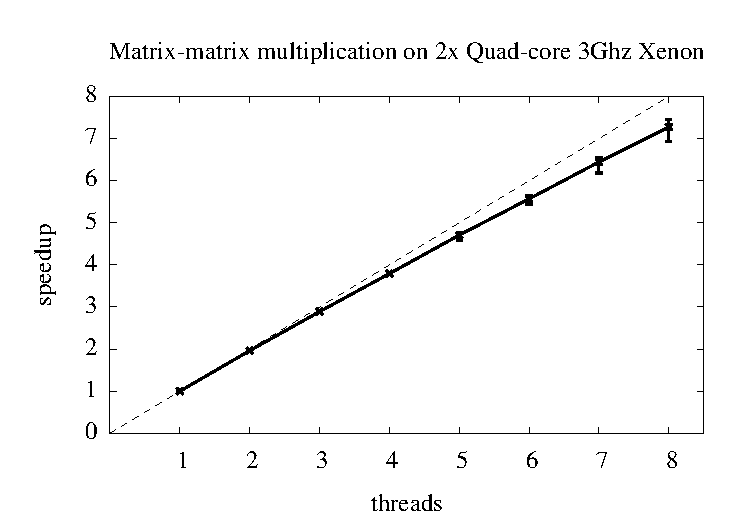
\includegraphics[width=0.5\textwidth]{figs/mmult-limitingfactor.pdf}

\hspace{-1em}
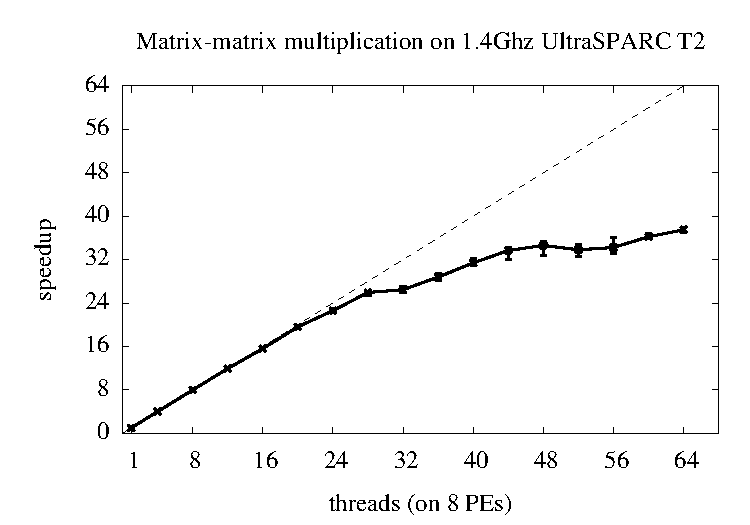
\includegraphics[width=0.5\textwidth]{figs/mmult-greyarea.pdf}

\caption{Matrix-matrix multiplication, size 1024x1024.}
\label{fig:mmult}
\end{figure}
 
\begin{figure}
\hspace{-1em}
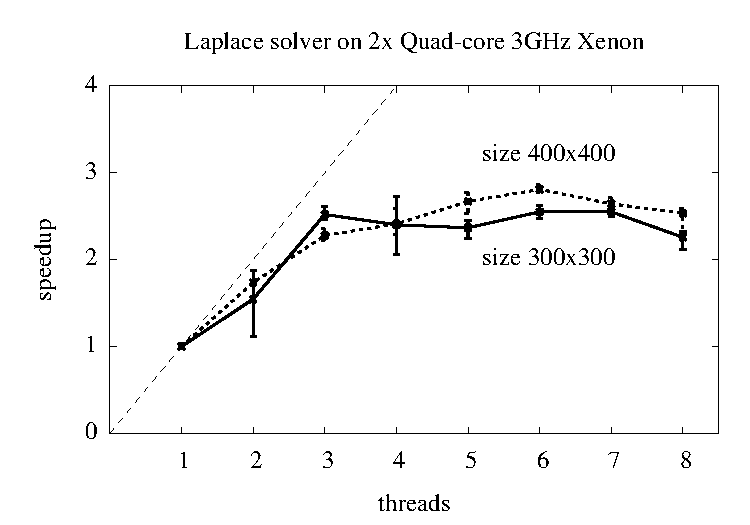
\includegraphics[width=0.5\textwidth]{figs/laplace-limitingfactor.pdf}

\hspace{-1em}
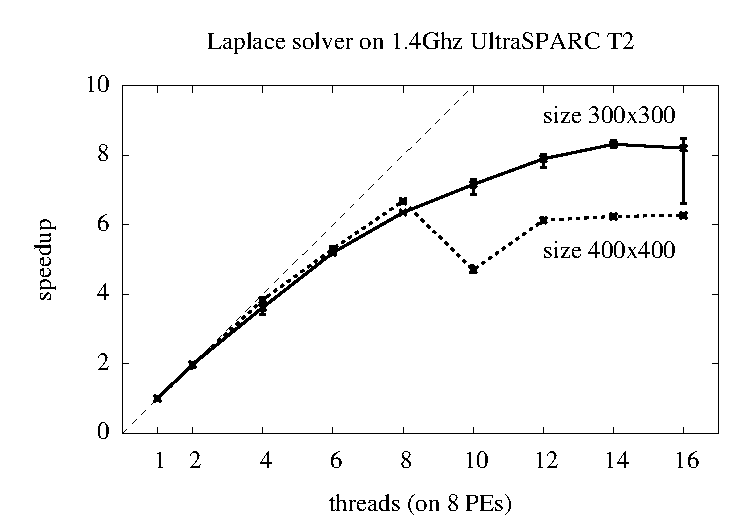
\includegraphics[width=0.5\textwidth]{figs/laplace-greyarea.pdf}

\caption{Laplace solver, 1000 iterations.}
\label{fig:laplace}
\end{figure}

\begin{figure}
\hspace{-1em}
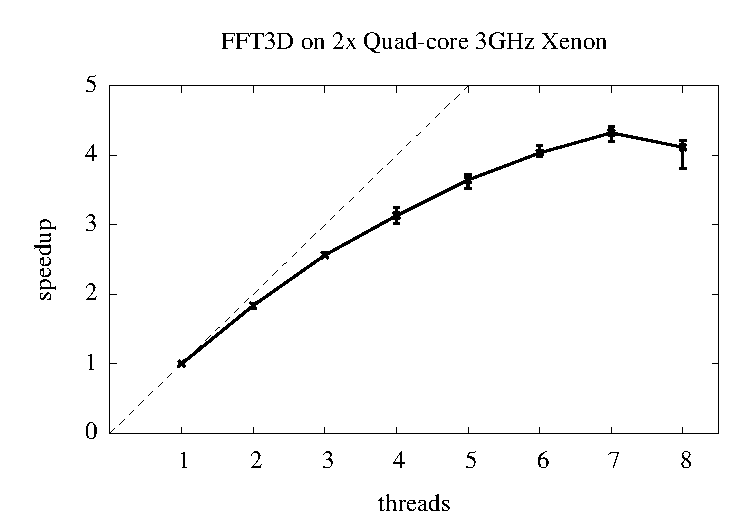
\includegraphics[width=0.5\textwidth]{figs/fft3D-limitingfactor.pdf}

\hspace{-1em}
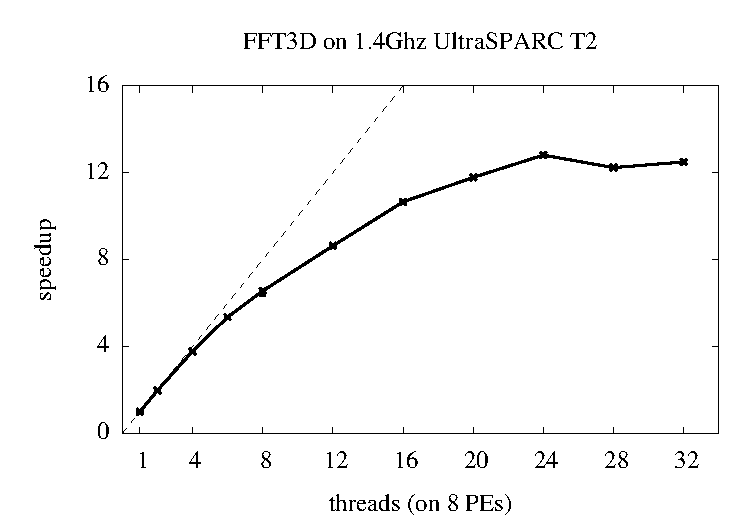
\includegraphics[width=0.5\textwidth]{figs/fft3D-greyarea.pdf}

\caption{3D Fast Fourier Transform, size 128x128x128}
\label{fig:fft}
\end{figure}


\subsection{Absolute performance}

Before discussing the parallel behaviour of our benchmarks, let us investigate
how Repa programs compare to hand-written C code when executed with only one thread.
The C matrix-matrix multiplication and Laplace solver are straightforwardly written
programs, while the FFT uses FFTW 3.2.2~\cite{frigo-johnson:fftw} in ``estimate'' mode.


Figure~\ref{fig:xeon-performance} shows the single threaded results together with
the fastest running times obtained through parallel execution. For matrix multiplication
and Laplace on the Xenon, Repa is slower than C when executed sequentially, but not by much.
FFTW uses a finely tuned in-place algorithm, which is significantly faster but more 
complicated than our own direct encoding of the Cooley-Tukey algorithm. We include
the numbers with FFTW for comparative purposes, but note that parallelism is no
substitute for a more efficient algorithm.

Compared with the Xenon, the results on the SPARC (Figure~\ref{fig:sparc-performance}) are quite different.
The SPARC T2 is a ``throughput'' machine, designed to execute workloads consisting of many
concurrent threads. It has half the clock rate of the Xenon, and does not exploit instruction
level parallelism. This shows in the fact that the single threaded C programs run about 10x slower
than their Xenon counterparts. The SPARC T2 also does not perform instruction reordering or use
speculative execution. GHC does not perform compile time scheduling to account for this, which
results in a larger gap between the single threaded C and Repa programs than on the Xenon.


% Unfortunately, GHC generates very poor code for SPARC architectures, making the
% performance difference between Repa programs and the
% corresponding C versions significanlty worse than on the Xeon. This is a
% temporary problem, however, as we expect the  new LLVM
% backend~\cite{LLVM:CGO04,LLVMbackend} to produce much faster code.
% Unfortunately, it has not been ported to the SPARC yet and
% sometimes generates incorrect code even on x86. We have only been able to use
% it for the Laplace benchmark on the Xeon machine but fully expect this
% situation to improve in the near future. In any case, when run on multiple
% threads the benchmarks are still able to achieve better performance than the
% sequential C programs.
% \finaltodo{Please give a more specific reference for the LLVM backend, or
%    leave out the paragraph (it does not make any contribution). review 3}

We have also compared the performance of the Laplace solver to an
alternative, purely sequential Haskell implementation based on unboxed,
mutable arrays running in the IO Monad (\verb|IOUArray|).
This version was about two
times slower than the Repa program, probably due to the overhead introduced by bounds
checking, which is currently not supported by our library. Note, however, that
bounds checking is unnecessary for many collective operations such as
\verb|map| and \verb|sum|, so even after we introduce it in Repa we still
expect to see better performance than a low-level, imperative implementation
based on mutable arrays.

%So, with the current
%implementation of our library, the trade off in the sequential case
%between \texttt{MArray} and our implementation is having to write the
%program in a fairly low-level imperative style, and having the safety
%of bounds checking on one hand, and having a faster program, written
%in a purely functional style on the other hand. We are currently
%planning to address bounds checking in a future version of our
%library, which can be done efficiently on the level of the underlying
%library, as shown in \TODO{ref to RL's vector lib}.
%

%  For
%  example, matrix-matrix multiplication was on the former only five
%  percent slower than the C implementation using the matrix
%  multiplication library function provided by the Accelerate library
%  on MacOS. On the SPARC, the Array version was three times slower
%  than the C version. With the new LLVM
%  backend~\cite{LLVM:CGO04,LLVMbackend} for GHC, we should be able to
%  overcome this problem. Indeed, with some preliminary benchmarks on
%  Xeon using LLVM we observed further performace
%  improvements. However, as there are currently still problems with
%  the correctness of the LLVM code produced, we cannot include the
%  numbers here. The numbers on the SPARC are of interest nevertheless,
%  as the architecture provides in general significantly better
%  scalability than the Xeon. We therefore include the figures
%  displaying the relative speedup of our benchmarks on the SPARC,
%  compared to the purely sequential Array version.  On the Xeon, we
%  show the absolute speed up, compared to the C version of the
%  program.

\subsection{Parallel behaviour}

The parallel performance of matrix multiplication is show in
Figure~\ref{fig:mmult}.\footnote{Yes, those really are the results in the first graph of the figure.} 
Each point shows the lowest, average, and highest speedups for ten consecutive runs.
Here, we get excellent scalability on both machines. On
the Xeon, we achieve a speedup of 7.2 with 8 threads. On the SPARC, 
it scales up to 64 threads with a peak speedup of 38.

Figure~\ref{fig:laplace} shows the relative speedups for the Laplace solver.
This program achieves good scalability on the SPARC, reaching a
speedup of 8.4 with 14 threads but performs much worse on the Xeon, stagnating
at a speedup of 2.5. As Laplace is memory bound, we attribute this behaviour 
to insufficient bandwidth on the Xeon machine. There is also some variation in the
speedups from run to run, which is more pronounced when using specific numbers of
threads. We attribute this to scheduling effects, in the hardware, OS, and GHC runtime system.

Finally, the parallel behaviour of the FFT implementation is shown in
Figure~\ref{fig:fft}. This program scales well on both machines, achieving a
relative speedup of 4.4 on with 7 threads on the Xeon and 12.7 on 14 threads on
the SPARC. Compared to the Laplace solver, this time the scalability is much better on
the Xenon but practically unchanged on the SPARC. Note that FFT is less memory 
intensive than Laplace. The fact that Laplace with a $300\times300$ matrix does not scale as well on 
the Xenon as it does on the SPARC supports our conclusion that this benchmark
suffers from lack of memory bandwidth. For Laplace with a $400\times400$ matrix on the SPARC, 
we suspect the sharp drop off after 8 threads is due to the added threads contending for 
cache. As written, the implementation
from Section \ref{sub:general_traversal} operates on a row-by-row basis. We expect
that changing to a block-wise algorithm would improve cache-usage and reduce the
bandwidth needed.
 


 

\section{Related Work}
%\finaltodo{n section 4.4, you seem to want some type of sized type,
%and sized type polymorphism. How does this system
%compare to the many attempts at using sized types as
%indices? review 2}

Array programming is a highly active research area so the amount of
related work is quite significant. In this section, we have to restrict
ourselves to discussing only a few most closely related approaches.

\subsection{Haskell array libraries}

Haskell 98 already defines an array type as part of its prelude which, in
fact, even provides a certain degree of shape polymorphism. These arrays can
be indexed by arbitrary types as long as they are instances of \verb|Ix|, a
type class which plays a similar role to our \verb|Shape|. This allows for
fully shape-polymorphic functions such as \verb|map|. However,
standard Haskell arrays do not support at-least constraints and rank generalisation
which are crucial for implementing highly expressive operations such as
\verb|sum| from Section~\ref{sec:at-least-rank}. This inflexibility precludes
many advanced uses of shape polymorphism described in this paper and makes
even unboxed arrays based on the same interface 
a bad choice for a parallel implementation.

% \TODO{Could Haskell standard arrays (at least the unboxed flavour) be
% implemented using the techniques in this paper --- i.e., could we just keep the
% Haskell array API?  Explain that Haskell arrays don't support ad-hoc shape polymorphism.}

Partly motivated by the shortcomings of standard arrays, numerous Haskell
array libraries have been proposed in recent years. These range from highly
specialised ones such as ByteString~\cite{coutts-etal:rewriting-haskell-strings}
to full-fledged DSLs for programming GPUs~\cite{lee-etal:gpu}.
However, these libraries do not provide the same
degree of flexibility and efficiency for manipulating regular arrays if they
support them at all.  Our own work on Data Parallel Haskell is of particular
relevance in this context as the work presented in this paper
shares many of its ideas and large parts of its implementation with that
project. Indeed, Repa can be seen as complementary to DPH. Both provide a
way of writing high-performance parallel programs but DPH supports irregular,
arbitrarily nested parallelism which requires it to sacrifice performance when
it comes to purely regular computations. One of the goals of this paper is to
plug that hole. Eventually, we intend to integrate Repa into DPH,
providing efficient support for both regular and irregular arrays in one framework.

\subsection{C++ Array Libraries}

Due to its powerful type system and its wide-spread use
in high-performance computing, C++ has a significant number of array libraries
that are both fast and generic. In particular,
Blitz++~\cite{veldhuizen:blitz} and
\verb|Boost.MultiArray|~\cite{boost:multiarray} feature
multidimensional arrays with a restricted form of shape polymorphism.
However, our library is much more flexible in this regard and also has the
advantage of a natural parallel implementation which neither of the two C++
libraries provide. Moreover, these approaches are inherently imperative while
we provide a purely functional interface which allows programs to be written
at a higher level of abstraction.

\subsection{Array Languages}

In addition to libraries, there exist a number of special-purpose array programming
languages. Of these, 
Single Assignment C (SAC)~\cite{scholz:SaC} has exerted the most influence on our work and
is the
closest in spirit as it is purely functional and strongly typed. SAC provides many of 
the same benefits as Repa: high-performance arrays
with shape polymorphism, expressive collective operations and
extensive optimisation based on \emph{with-loops}, a special-purpose language
construct for creating, traversing and reducing arrays. It also comes with a
rich library of standard
array and matrix operations which Repa has not yet acquired. 

%In addition to a rich standard library, the basic
%building blocks of SAC programs are \emph{with-loops}, a
%special-purpose language construct for constructing, traversing and reducing
%arrays. With-loops allow array programs to be written at a high level of
%abstraction and are also amenable to aggressive loop fusion which is crucial
%for achieving good performance.
%\finaltodo{  The with-loop in SAC is part of a core language, not intended for
%    programmer use but generated by the compiler. Programmers will
%    rather use standard operations (such as matrix arithmetics) overloaded
%    in shape-generic way in SAC (would be useful in repa as well).}

%While providing a similar level of expressiveness and performance, Repa
However, Repa
has the advantage of being integrated into a mainstream
functional language and not requiring specific compiler support. This allows
Repa programs to utilise the entire Haskell infrastructure and to
drop down to a very low level of abstraction if required in specific cases. This,
along with strong typing and purity, are also the advantages Repa has over
other array languages such as APL, J and Matlab~\cite{iso:apl,burke:j,amos:matlab}. 

% \TODO{ What is the relationship to
% \url{http://portal.acm.org/beta/citation.cfm?id=645390.651624} (Apart from using
% the term shape polymorphism). And is there anything in there related to rank
% generalisation?}

\paragraph{Acknowledgements.}
%
We are grateful to Arvind for explaining the importance of delaying index space transformations and thank Simon Winwood for comments on a draft.  We also thank the anonymous ICFP'10 reviewers for their helpful feedback on the paper. This research was funded in part by the Australian Research Council under grant number LP0989507.


\bibliographystyle{abbrvnat}
\bibliography{RArrays}

\end{document}
